% Paper B. IEEE conference format, at most 7 pages including references (the guide's limit). Venue not chosen yet.
% IEEE conference template (IEEEtran, conference, 10pt, no compsoc).
% Keep the anonymous author block until the venue is known; replace it with names if the venue is single-blind.
%
% THIS IS A SKELETON. Every \todo{} marks text the AUTHORS write. The guide that says what goes where is
% paper_b/README.md -> 02_section_guide.md (section content), 03_figures_tables.md (figures/captions),
% 05_numbers.md (every number you may quote, with its source). Tables below already hold the measured
% numbers (from paper_b/figure_data/*.csv); check them against 05_numbers.md if you edit them.
%
% Compile on Overleaf: New Project -> Upload Project (zip of paper_b/latex/), or copy these files into the
% "IEEE Conference Template" project. Bibliography: BibTeX with refs.bib (IEEEtran style).

\documentclass[conference,10pt]{IEEEtran}
\IEEEoverridecommandlockouts
\usepackage{cite}
\usepackage{amsmath,amssymb}
\usepackage{graphicx}
\usepackage{booktabs}
\usepackage{url}
\usepackage{xcolor}
\newcommand{\todo}[1]{\textcolor{red}{[TODO: #1]}}

\begin{document}

\title{\todo{title: see 01\_story\_and\_claims.md, "Title ingredients"}}

\author{\IEEEauthorblockN{Anonymous Author(s)}
\IEEEauthorblockA{Anonymous Institution}}

\maketitle

\begin{abstract}
\todo{150--200 words; content points in 01\_story\_and\_claims.md, "Abstract content points". Write it LAST.}
\end{abstract}

\begin{IEEEkeywords}
self-adaptive systems, self-healing, monitoring, tail latency, microservices, edge computing
\end{IEEEkeywords}

% =====================================================================================================
\section{Introduction}\label{sec:intro}
\todo{$\approx$0.75 page. 02\_section\_guide.md, Section 1: problem, setting, RQ1--RQ3, contributions list.}

% =====================================================================================================
\section{Setting}\label{sec:setting}
\todo{$\approx$0.75 page. 02\_section\_guide.md, Section 2 and 04\_methodology\_facts.md (testbed, control loop, signals, calibration rule).}

\begin{figure}[t]
  \centering
  % Replace this box with: \includegraphics[width=\columnwidth]{figures/testbed.pdf}
  \fbox{\parbox{0.9\columnwidth}{\centering\vspace{1.2cm}
  Fig.~1 placeholder: testbed and the three measurement points.\\
  Drawing spec: 03\_figures\_tables.md, ``Fig.~1''.\vspace{1.2cm}}}
  \caption{\todo{caption facts in 03\_figures\_tables.md, Fig.~1}}
  \label{fig:testbed}
\end{figure}

\begin{table}[t]
  \centering
  \caption{\todo{caption: the three SLA latency signals compared}}
  \label{tab:signals}
  \small
  \begin{tabular}{@{}lll@{}}
    \toprule
    Signal & Measured at & Path included \\
    \midrule
    Client p99 & load generator (B) & app + wireless link \\
    Server p95/p99 & frontend logs (A) & app only \\
    Ping p99 & ICMP, B$\rightarrow$A & wireless link only \\
    \bottomrule
  \end{tabular}
\end{table}

% =====================================================================================================
\section{Method}\label{sec:method}
\todo{$\approx$0.75 page. 02\_section\_guide.md, Section 3 and 04\_methodology\_facts.md (tick-aligned collection, stall detection, bootstrap of quantiles, decision view).}

% =====================================================================================================
\section{Results}\label{sec:results}

\subsection{RQ1: Separating the noise sources}\label{sec:rq1}
\todo{$\approx$0.8 page. 02\_section\_guide.md, 4.1; Fig.~\ref{fig:decomposition}, Fig.~\ref{fig:timeseries}, Table~\ref{tab:stalls}.}

\begin{figure*}[t]
  \centering
  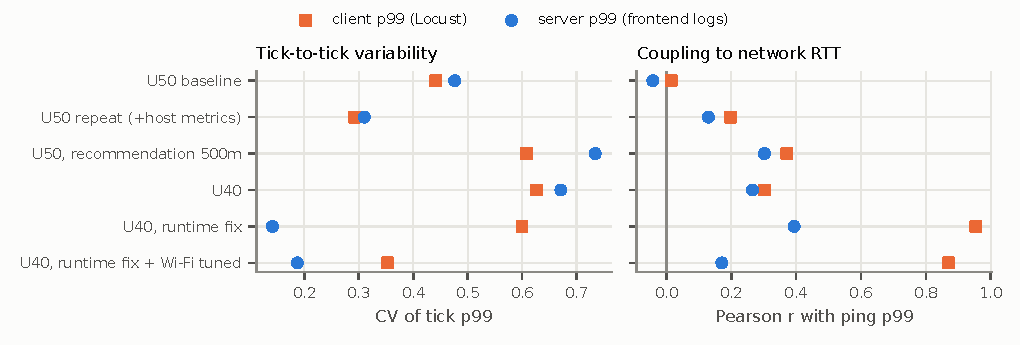
\includegraphics[width=\textwidth]{figures/b1_decomposition.pdf}
  \caption{\todo{caption facts in 03\_figures\_tables.md, Fig.~b1}}
  \label{fig:decomposition}
\end{figure*}

\begin{figure}[t]
  \centering
  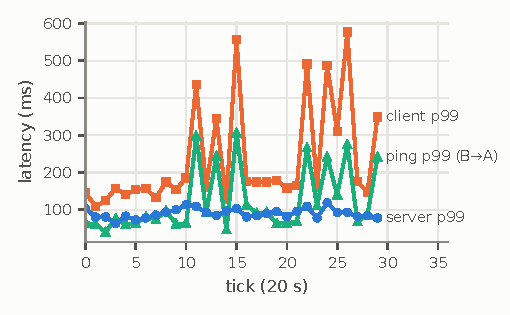
\includegraphics[width=\columnwidth]{figures/b2_timeseries_treatA.pdf}
  \caption{\todo{caption facts in 03\_figures\_tables.md, Fig.~b2}}
  \label{fig:timeseries}
\end{figure}

\begin{table}[t]
  \centering
  \caption{\todo{caption: sub-second stall events before/after the runtime fix (U40)}}
  \label{tab:stalls}
  \begin{tabular}{@{}lrr@{}}
    \toprule
    & Before fix & After fix \\
    \midrule
    Requests observed & 16{,}639 & 17{,}141 \\
    Requests $>$ 500\,ms & 448 (2.7\,\%) & 0 \\
    Stall events (per min) & 37 (7.0) & 0 (0) \\
    Median event duration & 0.81\,s & -- \\
    Events with a ping spike & 0 & 0 \\
    \bottomrule
  \end{tabular}
\end{table}

\subsection{RQ2: Estimator noise and the tail-sample rule}\label{sec:rq2}
\todo{$\approx$0.6 page. 02\_section\_guide.md, 4.2; Fig.~\ref{fig:estimator}.}

\begin{figure}[t]
  \centering
  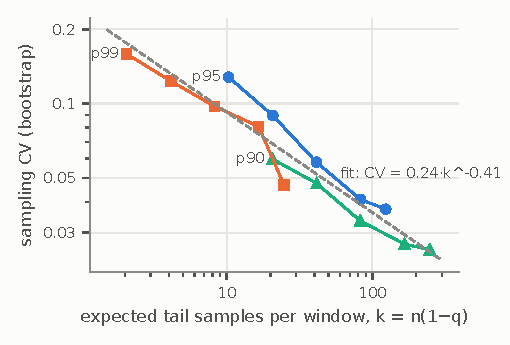
\includegraphics[width=\columnwidth]{figures/b3_estimator_noise.pdf}
  \caption{\todo{caption facts in 03\_figures\_tables.md, Fig.~b3}}
  \label{fig:estimator}
\end{figure}

\subsection{RQ3: What the controller can see}\label{sec:rq3}
\todo{$\approx$1.0 page. 02\_section\_guide.md, 4.3; Table~\ref{tab:inflation}, Fig.~\ref{fig:detect}, Table~\ref{tab:runbook}; transport numbers.}

\begin{table}[t]
  \centering
  \caption{\todo{caption: threshold from the same calibration rule, per signal; held-out false breaches}}
  \label{tab:inflation}
  \begin{tabular}{@{}llrrr@{}}
    \toprule
    Run & Signal & CV & Threshold & Thr./median \\
    \midrule
    keep-alive, U33 & server p95 & 0.29 & 60\,ms & 2.4$\times$ \\
                    & client p99 & 1.24 & 350\,ms & 3.2$\times$ \\
    final, U30      & server p95 & 0.24 & 70\,ms & 2.9$\times$ \\
                    & client p99 & 0.75 & 1100\,ms & 5.7$\times$ \\
    \bottomrule
  \end{tabular}
\end{table}

\begin{figure}[t]
  \centering
  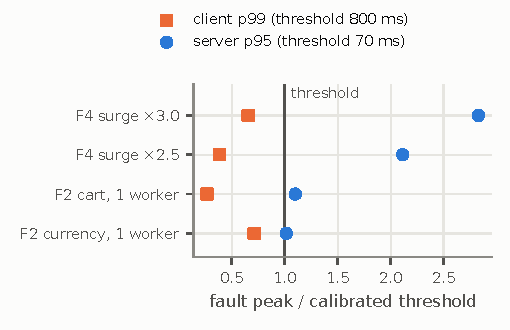
\includegraphics[width=\columnwidth]{figures/b4_detectability.pdf}
  \caption{\todo{caption facts in 03\_figures\_tables.md, Fig.~b4}}
  \label{fig:detect}
\end{figure}

\begin{table}[t]
  \centering
  \caption{\todo{caption: detection in the first two fault ticks (latency over threshold OR failures $>$1\,\%), runbook episodes}}
  \label{tab:runbook}
  \begin{tabular}{@{}lrrr@{}}
    \toprule
    Fault & Episodes & Server p95 & Client p99 \\
    \midrule
    F1 bad deploy & 24 & 24 & 24 \\
    F2 CPU stress & 29 & 27 & 3 \\
    F3 scale to zero & 33 & 33 & 33 \\
    F4 traffic surge & 29 & 29 & 5 \\
    \midrule
    \multicolumn{2}{@{}l}{Fault-free ticks over threshold} & 6/421 & 17/421 \\
    \bottomrule
  \end{tabular}
\end{table}

% =====================================================================================================
\section{Guidelines}\label{sec:guidelines}
\todo{$\approx$0.45 page. 02\_section\_guide.md, Section 5: numbered guidelines, each tied to a result above.}

% =====================================================================================================
\section{Threats to Validity}\label{sec:threats}
\todo{$\approx$0.25 page. 02\_section\_guide.md, Section 6.}

% =====================================================================================================
\section{Related Work}\label{sec:related}
\todo{$\approx$0.45 page. 06\_references.md: groups, what each paper does, how we differ. Cite only verified entries.}

% =====================================================================================================
\section{Conclusion}\label{sec:conclusion}
\todo{$\approx$0.2 page. One sentence per RQ; artifact availability (anonymized link).}

% =====================================================================================================
\section*{Acknowledgment}
\todo{AI-assistance disclosure, required by IEEE policy; content points in 07\_format\_and\_submission.md. Keep it anonymous.}

% TEMPORARY: \nocite{*} lists every refs.bib entry so the skeleton compiles before any \cite exists
% (an empty bibliography is a LaTeX error). DELETE this line once the text cites its references, so only
% cited, verified references appear.
\nocite{*}
\bibliographystyle{IEEEtran}
\bibliography{refs}

\end{document}
